\section{\texorpdfstring{Obvody kombinační logiky}{Obvody kombinacni logiky}}

% =====================================================================================================================
	\begin{frame}
    \frametitle{Sčítačka - poloviční}
		
		\begin{minipage}[t][\textheight][t]{0.45\textwidth}
		\vspace{10mm}
		\begin{center}
			\begin{tabular}{ c c | c c }
				$X$ & $Y$ & $SUM$ & $CARRY$\\
				\hline
				0 & 0 & 0 & 0 \\
				0 & 1 & 1 & 0 \\
				1 & 0 & 1 & 0 \\
				1 & 1 & 0 & 1 \\
			\end{tabular}
		\end{center}

		\end{minipage}
		\begin{minipage}[t][\textheight][t]{0.45\textwidth}
    \vspace{10mm}
		
			\begin{itemize}
				\item Realizuje sčítání dvou bitů,
				\item dva vstupy pro proměnné,
				\item dva výstupy:
				
				\begin{itemize}
					\item výsledek součtu a
					\item přenos do vyššího řádu,
				\end{itemize}
				
				\item součet lze realizovat pomocí hradla XOR,
				\item přenos přesně odpovídá hradlu AND.
			\end{itemize}

		\end{minipage}
		
	\end{frame}
	
% =====================================================================================================================
	\begin{frame}
    \frametitle{Sčítačka - poloviční, zapojení}
		
		\begin{minipage}[t][0.5\textheight][t]{0,45\textwidth}
		
		\textbf{SUM - XOR}
		\begin{center}
			\begin{karnaugh-map}[2][2][1][$Y$][$X$]
				\minterms{1,2}
				
				% ====== vlastní čáry ======

				% A = 1 (druhý řádek)
				\draw[very thick] (-0.15,1) -- (-0.15,0);

				% B = 1 (sloupce 3 a 4)
				\draw[very thick] (1,2.15) -- (2,2.15);

			\end{karnaugh-map}
		\end{center}

		\end{minipage}
		\begin{minipage}[t][0.5\textheight][t]{0,45\textwidth}
		
		\textbf{CARRY - AND}
		\begin{center}
			\begin{karnaugh-map}[2][2][1][$Y$][$X$]
				\minterms{3}
				% ====== vlastní čáry ======

				% A = 1 (druhý řádek)
				\draw[very thick] (-0.15,1) -- (-0.15,0);

				% B = 1 (sloupce 3 a 4)
				\draw[very thick] (1,2.15) -- (2,2.15);

			\end{karnaugh-map}
		\end{center}

		\end{minipage}
		\begin{minipage}[t][0.4\textheight][t]{\textwidth}

		
		\begin{center}
			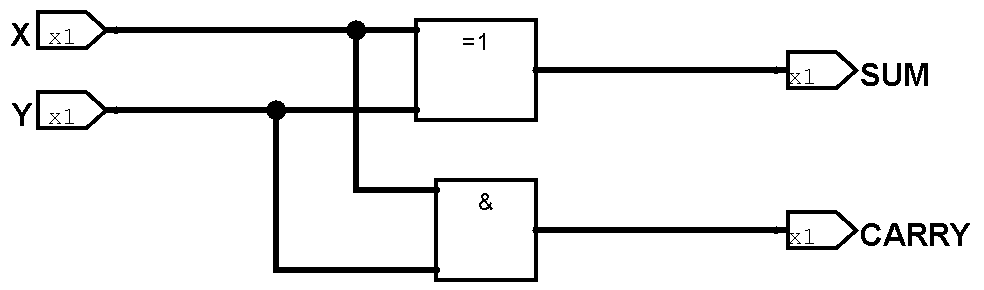
\includegraphics[width=\textheight]{fig/half_adder.png}
		\end{center}

		\end{minipage}
		
	\end{frame}
	
% =====================================================================================================================
	\begin{frame}
    \frametitle{Sčítačka - úplná}
		
		\begin{minipage}[t][\textheight][t]{0.5\textwidth}
		\vspace{10mm}
		\begin{center}
			\begin{tabular}{ c c c | c c }
				$CIN$ & $X$ & $Y$ & $SUM$ & $COUT$\\
				\hline
				0 & 0 & 0 & 0 & 0 \\
				0 & 0 & 1 & 1 & 0 \\
				0 & 1 & 0 & 1 & 0 \\
				0 & 1 & 1 & 0 & 1 \\
				1 & 0 & 0 & 1 & 0 \\
				1 & 0 & 1 & 0 & 1 \\
				1 & 1 & 0 & 0 & 1 \\
				1 & 1 & 1 & 1 & 1 \\
			\end{tabular}
		\end{center}

		\end{minipage}
		\begin{minipage}[t][\textheight][t]{0.45\textwidth}

			\begin{itemize}
				\item Realizuje sčítání dvou bitů s respektováním předchozího přenosu,
				\item tři vstupy:
				
				\begin{itemize}
					\item dva pro proměnné,
					\item jeden pro přenos z nižšího řádu,
				\end{itemize}
				
				\item dva výstupy:
				
				\begin{itemize}
					\item výsledek součtu a
					\item přenos do vyššího řádu,
				\end{itemize}
				
				\item lze snadno realizovat pomocí dvou polovičních sčítaček.
			\end{itemize}

		\end{minipage}
		
	\end{frame}
	
% =====================================================================================================================
	\begin{frame}
    \frametitle{Sčítačka - úplná, zapojení}
		
		
		\begin{center}
			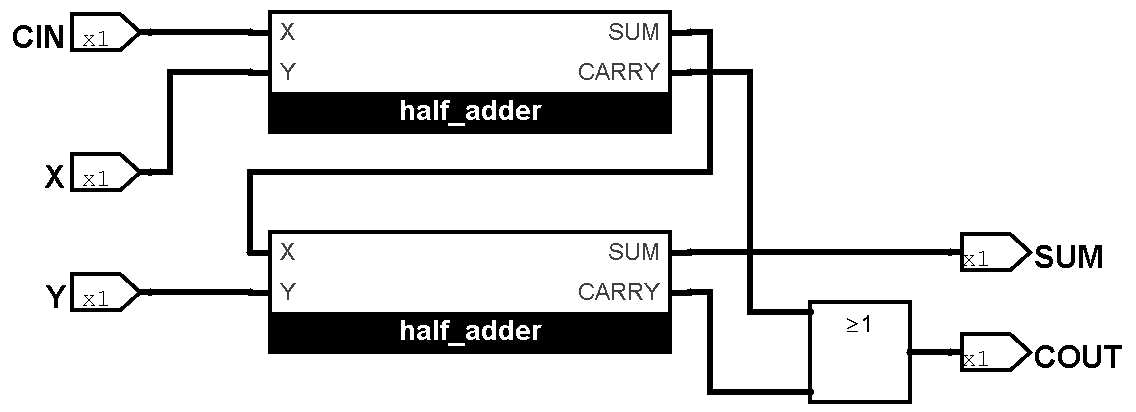
\includegraphics[width=1.00\textwidth]{fig/full_adder.png}
		\end{center}
		
		Hradlo \textbf{OR}: 
		
		\begin{itemize}
			\item přenos vznikne při $CIN + X$ \textbf{NEBO} při $(CIN + X) + Y$.
		\end{itemize}
		
	\end{frame}
	
% =====================================================================================================================
	\begin{frame}
    \frametitle{Dekodér}

			\begin{itemize}
				\item Převádí kombinaci vstupů na specifickou kombinaci výstupů,
				\item má více jak dva vstupy a více jak dva výstupy
				\item lze se s ním setkat například u:
				
				\begin{itemize}
					\item dekodér BCD kódu - přepis hodnoty do dekadické formy po 4 bitech,
					\item sedmisegmentový dekodér,
					\item dekodér 1 z 8 (viz dále).
				\end{itemize}
			\end{itemize}
		\vspace{5mm}
		
		\begin{minipage}[t][0.3\textheight][t]{0.5\textwidth}
			\textbf{B}inary \textbf{C}oded \textbf{D}ecimal
			
			\vspace{2mm}
			Dekadický zápis v binární formě:
			
			\begin{itemize}
				\item 4 bity pro 1 cifru,
				\item platné hodnoty 0 až 9.
			\end{itemize}
			
		\end{minipage}
		\begin{minipage}[t][0.3\textheight][t]{0.45\textwidth}
		
			\vspace{5mm}
			\begin{center}
				Číslo $(47)_{10}$
				\begin{tabular}{ | c | c | c | c || c | c | c | c | }
					\hline
					0 & 1 & 0 & 0 & 0 & 1 & 1 & 1 \\ \hline
				\end{tabular}
			\end{center}
			
		\end{minipage}
	\end{frame}
	
% =====================================================================================================================
	\begin{frame}
    \frametitle{Dekodér - 1 z 8}

		
		\begin{center}
			\begin{tabular}{ c c c | c c c c c c c c }
			  $A2$ & $A1$ & $A0$ & $Y0$ & $Y1$ & $Y2$ & $Y3$ & $Y4$ & $Y5$ & $Y6$ & $Y7$ \\
				\hline
				0 & 0 & 0 &  1 & 0 & 0 & 0 & 0 & 0 & 0 & 0 \\
				0 & 0 & 1 &  0 & 1 & 0 & 0 & 0 & 0 & 0 & 0 \\
				0 & 1 & 0 &  0 & 0 & 1 & 0 & 0 & 0 & 0 & 0 \\
				0 & 1 & 1 &  0 & 0 & 0 & 1 & 0 & 0 & 0 & 0 \\
				1 & 0 & 0 &  0 & 0 & 0 & 0 & 1 & 0 & 0 & 0 \\
				1 & 0 & 1 &  0 & 0 & 0 & 0 & 0 & 1 & 0 & 0 \\
				1 & 1 & 0 &  0 & 0 & 0 & 0 & 0 & 0 & 1 & 0 \\
				1 & 1 & 1 &  0 & 0 & 0 & 0 & 0 & 0 & 0 & 1 \\
			\end{tabular}
		\end{center}
		
		\begin{itemize}
			\item Každý výstup je aktivní právě při jedné kombinaci vstupů,
			\item realizuje se pomocí hradel AND (NAND pro inverzní logiku),
			\item je to základní stavební kámen multiplexoru a demultiplexoru.
		\end{itemize}
		
	\end{frame}
	
	% =====================================================================================================================
	\begin{frame}
    \frametitle{Dekodér - 1 z 8, zapojení}
    
    \begin{minipage}[t][\textheight][t]{0.5\textwidth}
      \vspace{-0.7\baselineskip}
			\begin{center}
        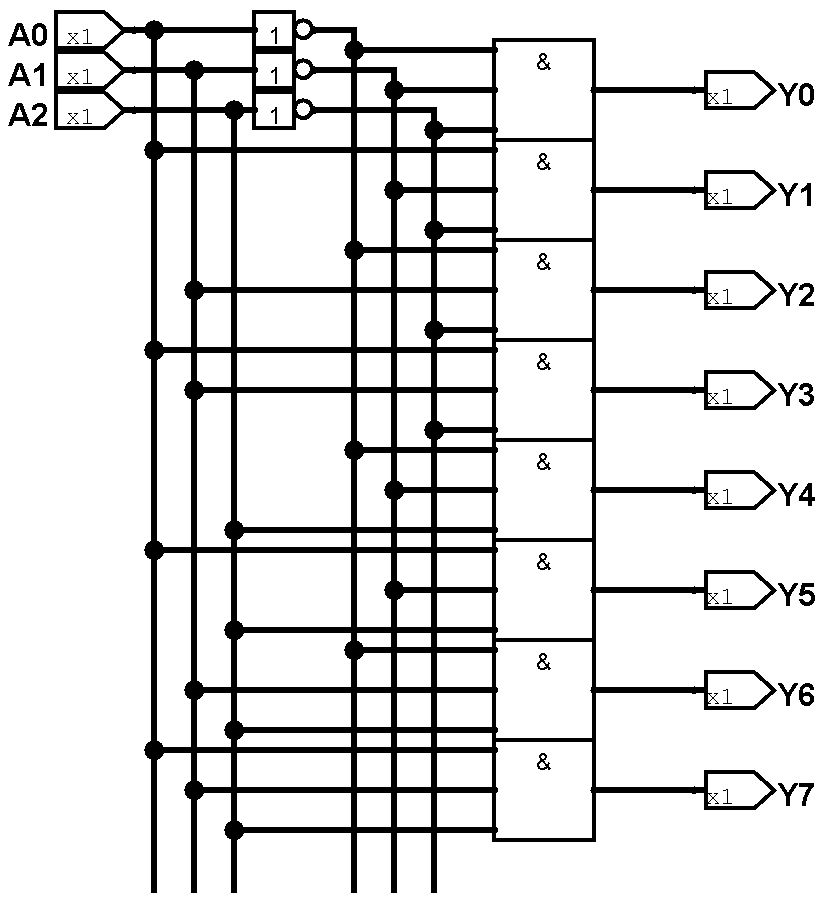
\includegraphics[scale=0.2]{fig/decoder_1_of_8.png}
      \end{center}
			
		\end{minipage}
		\begin{minipage}[t][\textheight][t]{0.45\textwidth}
      \vspace{-0.7\baselineskip}
      \begin{itemize}
        \item Jeden minterm pro řádek tabulky:
        \begin{align*}
          Y0 =& \bar{A2}\bar{A1}\bar{A0} \\
          Y1 =& \bar{A2}\bar{A1}A0 \\
          Y2 =& \bar{A2}A1\bar{A0} \\
          Y3 =& \bar{A2}A1A0 \\
          Y4 =& A2\bar{A1}\bar{A0} \\
          Y5 =& A2\bar{A1}A0 \\
          Y6 =& A2A1\bar{A0} \\
          Y7 =& A2A1A0 \\
        \end{align*}
      \end{itemize}
			
		\end{minipage}
		
	\end{frame}
	
	% =====================================================================================================================
	\begin{frame}
    \frametitle{Multiplexer / demultiplexer}

		
		\begin{itemize}
			\item Jsou to ve své podstatě digitální přepínače:
			
			\begin{itemize}
				\item \textbf{MULTIPLEXER:} připojení jednoho z N vstupů na jeden výstup,
				\item \textbf{DEMULTIPLEXER:} připojení jednoho vstupu na jeden z N výstupů.
			\end{itemize}
		\end{itemize}
		
		\begin{minipage}[t][0.65\textheight][t]{0.5\textwidth}
						
			
			\begin{center}
				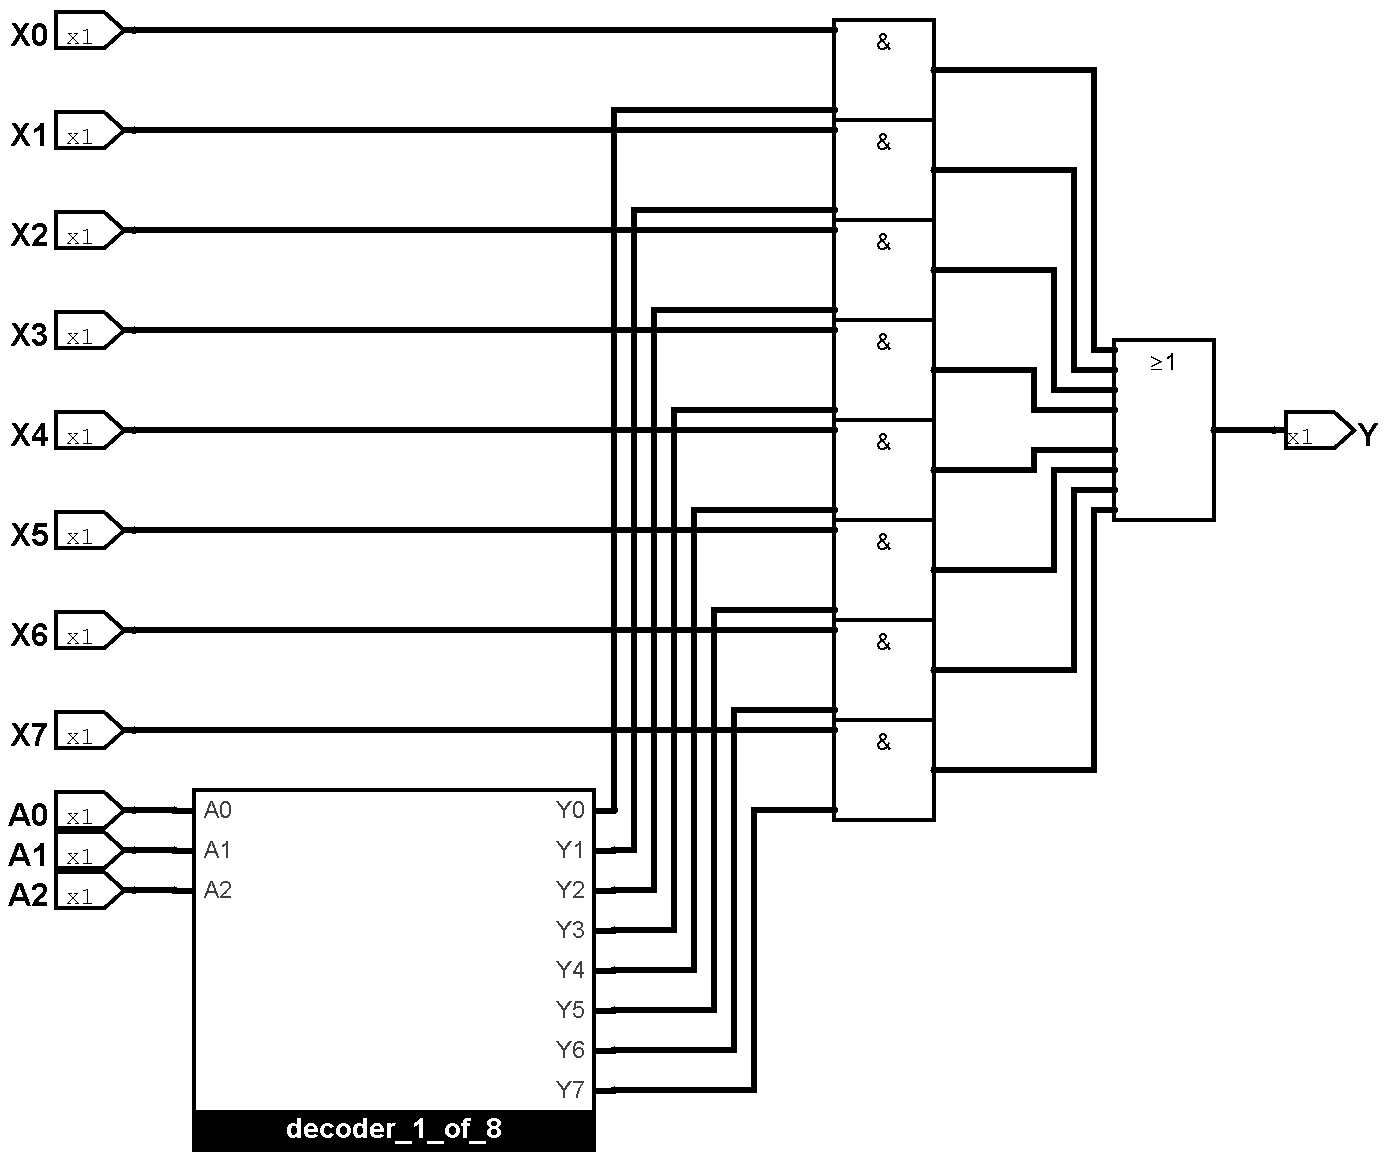
\includegraphics[scale=0.12]{fig/mux_8.png}
				\textbf{MULTIPLEXER}
			\end{center}
			
		\end{minipage}
		\begin{minipage}[t][0.65\textheight][t]{0.45\textwidth}
		
			\begin{center}
				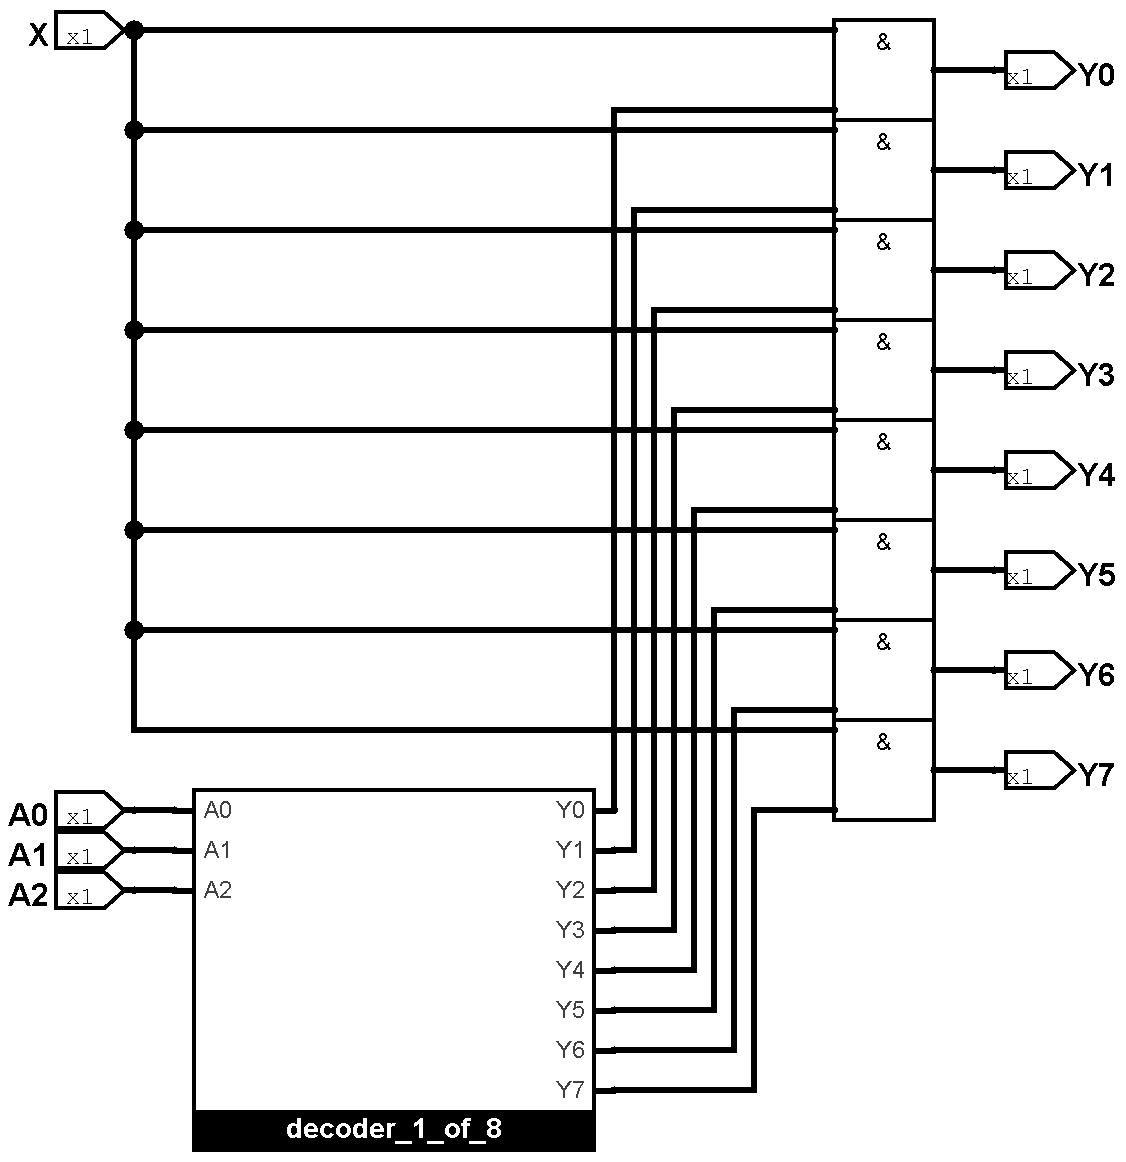
\includegraphics[scale=0.12]{fig/demux_8.png}
				\textbf{DEMULTIPLEXER}
			\end{center}
			
		\end{minipage}
		
	\end{frame}

% =====================================================================================================================
	\begin{frame}
    \frametitle{Používané symboly}
		
		\begin{minipage}[t][\textheight][t]{0.5\textwidth}
		
		\vspace{1mm}
		\begin{center}
			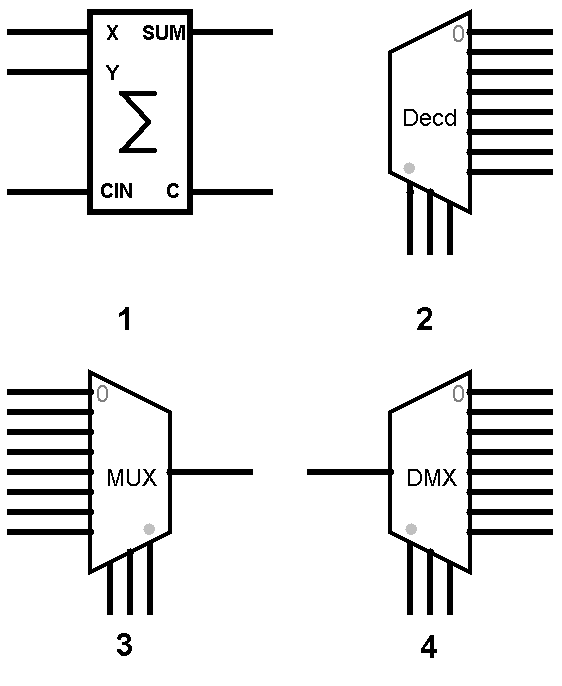
\includegraphics[width=1.00\textwidth]{fig/symboly.png}
		\end{center}

		\end{minipage}
		\begin{minipage}[t][\textheight][t]{0.45\textwidth}

		\vspace{6mm}
			
			\begin{enumerate}
				\item Sčítačka,
				\item dekodér,
				\item multiplexer,
				\item demultiplexer.
			\end{enumerate}
			
		\vspace{4mm}
		\small
			\begin{itemize}
				\item Adresní vstupy se kreslí dolů.
				\item Ve schématu je nutné označit adresní bit 0 a vstupní nebo výstupní bit 0.
			\end{itemize}

		\end{minipage}
		
	\end{frame}